Conforme dito no capitulo \ref{chap:mati} o trabalho foi divido em 4 etapas, nas quais a primeira etapa consistiu no estudo dos DPDs e nos métodos de modelagem deles, a segunda etapa consistiu na implementação desta modelagem em software, que foi optado em utilizar o python, a etapa 3 que consiste na implementação do modelo de DPD escolhido em hardware ultilizando a linguagem VHDL e finalmente na quarta etapa e feita o design do circuito integrado do circuito integrado.
Neste capitulo serão exibidos os resultados das etapas 2 ja que a etapa 1 cosiste no pesquisa bibliográfica e as etapas 3 e 4 serão desenvolvidas na segunda etapa do projeto.

\section{Etapa 2}
A etapa 2 consiste na modelagem do PA em software para posteriormente ser feito a modelagem do DPD, e finalmente ser feito o levantamento da quantidade de bits necessarios para a implementação do DPD em hardware minimizando os erros de quantização. 
O resultado desse levantamento esta presente no grafico na figura \ref{fig:bits}, onde observa-se que a partir de 7 bits de resolução não tem uma melhora expressiva no NMSE do sinal.

\begin{figure}[ht!]
    \centering
    \captionsetup{justification=centering}
    \caption*{Fonte: Autor}
    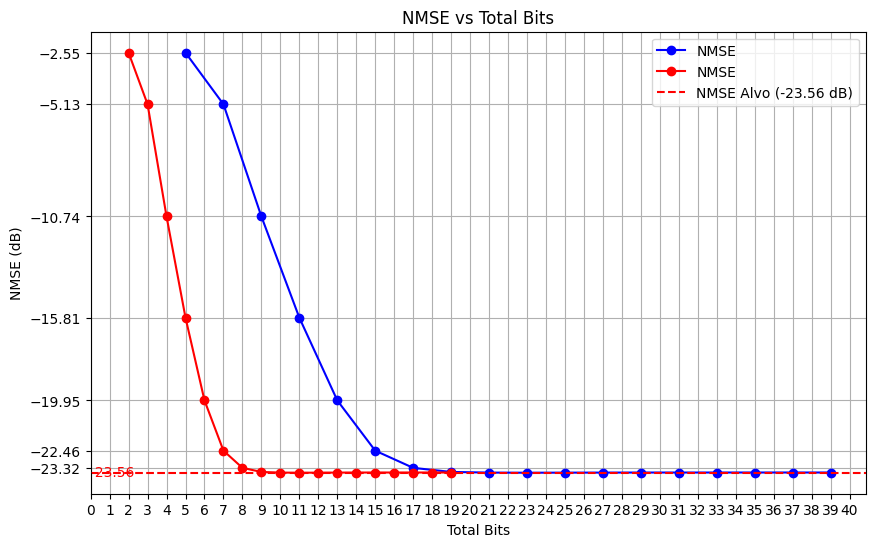
\includegraphics[width=0.5\textwidth]{bits.png}
    \caption{Grafico Numero de bits x NMSE}
    \label{fig:bits}
\end{figure}


